\documentclass[tikz,border=3mm]{standalone}
\usetikzlibrary{arrows.meta,calc}
\begin{document}
\pagecolor{white}
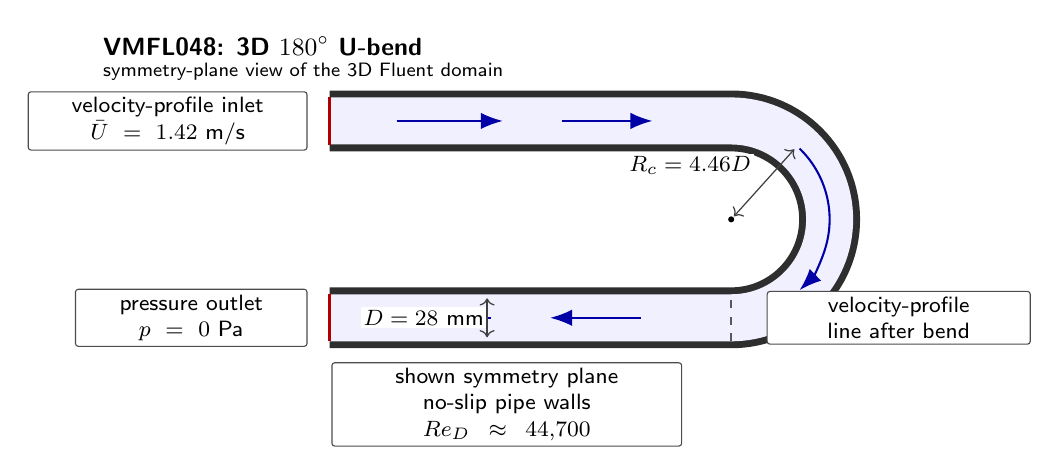
\begin{tikzpicture}[
  font=\sffamily\footnotesize,
  flow/.style={-{Latex[length=2.8mm]}, line width=0.75pt, draw=blue!65!black},
  dim/.style={<->, line width=0.45pt, draw=black!75, shorten <=1.5pt, shorten >=1.5pt},
  section/.style={draw=red!70!black, line width=1.1pt},
  profile/.style={draw=black!65, dashed, line width=0.85pt},
  bc/.style={draw=black!70, fill=white, rounded corners=1pt, inner sep=2pt, align=center}
]

\node[font=\sffamily\bfseries\small, anchor=west] at (0.10,4.75)
  {VMFL048: 3D $180^\circ$ U-bend};
\node[font=\sffamily\scriptsize, anchor=west] at (0.10,4.42)
  {symmetry-plane view of the 3D Fluent domain};

\def\r{1.25}
\def\cx{8.20}
\def\cy{2.55}
\def\w{0.30}
\def\xleft{3.10}
\def\ytop{\cy+\r}
\def\ybot{\cy-\r}

\draw[black!82, line width=22pt, line cap=butt, line join=round]
  (\xleft,\ytop) -- (\cx,\ytop) arc[start angle=90,end angle=-90,radius=\r] -- (\xleft,\ybot);
\draw[blue!6, line width=17pt, line cap=butt, line join=round]
  (\xleft,\ytop) -- (\cx,\ytop) arc[start angle=90,end angle=-90,radius=\r] -- (\xleft,\ybot);

% Boundary planes and labels.
\draw[section] (\xleft,\ytop-\w) -- (\xleft,\ytop+\w);
\draw[section] (\xleft,\ybot-\w) -- (\xleft,\ybot+\w);
\node[bc, anchor=east, text width=34mm] at (\xleft-0.28,\ytop)
  {velocity-profile inlet\\$\bar{U}=1.42$ m/s};
\node[bc, anchor=east, text width=28mm] at (\xleft-0.28,\ybot)
  {pressure outlet\\$p=0$ Pa};

% Flow direction.
\draw[flow] (3.95,\ytop) -- (5.30,\ytop);
\draw[flow] (6.05,\ytop) -- (7.20,\ytop);
\draw[flow] ({\cx+\r*cos(46)},{\cy+\r*sin(46)}) arc[start angle=46,end angle=-46,radius=\r];
\draw[flow] (7.05,\ybot) -- (5.90,\ybot);
\draw[flow] (5.15,\ybot) -- (3.85,\ybot);

% Bend radius and diameter.
\coordinate (bendcenter) at (\cx,\cy);
\coordinate (radiuspoint) at ({\cx+\r*cos(48)},{\cy+\r*sin(48)});
\draw[dim] (bendcenter) -- (radiuspoint);
\node[fill=white, inner sep=1pt, anchor=east] at ($(bendcenter)!0.54!(radiuspoint)+(-0.16,0.18)$)
  {$R_c=4.46D$};
\fill[black] (bendcenter) circle (1.1pt);

\draw[dim] (5.10,\ybot-\w) -- node[left, fill=white, inner sep=1pt]
  {$D=28$ mm} (5.10,\ybot+\w);

% Velocity-profile extraction line.
\draw[profile] (\cx,\ybot-\w) -- (\cx,\ybot+\w);
\node[bc, anchor=west, text width=32mm] at (\cx+0.45,\ybot)
  {velocity-profile\\line after bend};

\node[bc, text width=43mm] at (5.35,0.20)
  {shown symmetry plane\\no-slip pipe walls\\$Re_D\approx44{,}700$};

\end{tikzpicture}
\end{document}
